\chapter{HSRP}

\section{Operations}

One way to prevent a single point of failure at the default gateway is to implement a virtual router. Specifically, multiple routers are configured by First Hop Redundancy Protocol (FHRP) to work together as an illusion of a single router to the hosts on the LAN. \\

There are many options available for FHRP: HSRP (Cisco), GLBP (Cisco), VRRP (non-proprietary), IRDP (non-proprietary). This topic only introduces Hot Standby Router Protocol (HSRP), designed by Cisco. This protocol allows for gateway redundancy without any additional configuration on end devices.\\
 
HSRP selects exactly one active router and one standby router. The active router will act as the default gateway for end devices. The default gateway address is a virtual IPv4 address along with a virtual MAC address that is shared amongst both HSRP routers. End devices use this virtual IPv4 address as their default gateway address.(See figure \ref{HSRP-topology}). The virtual IPv4 address is configured by the network administrator. The virtual MAC address is created automatically.

\begin{figure}[hbtp]
\centering
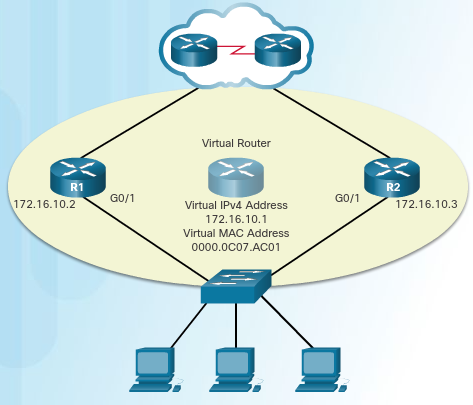
\includegraphics[width=0.6\textwidth]{pictures/HSRP.png}
\caption{HSRP topology}
\label{HSRP-topology}
\end{figure}

\section{Priority}

HSRP priority can be used to determine the active router. The router with the highest HSRP priority will become the active router. By default, the HSRP priority is 100. If the priorities are equal, the router with the numerically highest IPv4 address is elected as the active router.

\section{Preemption}

By default, after a router becomes the active router, it will remain the active router even if another router comes online with a higher HSRP priority. This means that the router which boots up first will become the active router if there are no other routers online during the election process.\\

To force a new HSRP election process, preemption must be enabled. Preemption is the ability of an HSRP router to trigger the re-election process. With preemption enabled, a router that comes online with a higher HSRP priority will assume the role of the active router. Preemption only allows a router to become the active router if it has a higher priority. However, a router with equal priority will not preempt an active router, even if it has higher IPv4 address.

\section{States and timers}

When an interface is configured with HSRP, it exchanges HSRP hello packets to determine which router is active. Hello packets are sent to the HSRP group multicast address every 3 seconds (hello timer), by default. The standby router will become active if it does not receive a hello message from the active router after 10 seconds (hold timer). To avoid increased CPU usage and unnecessary standby state changes, do not set the hello timer below 1 second or the hold timer below 4 seconds.

\section{Configuration}
Complete the following steps to configure HSRP:
\begin{enumerate}
    \item Configure HSRP version 2.
    \item Configure the virtual IP address for the group.
    \item Configure the priority for the desired active router to be greater than 100.
    \item Configure the active router to preempt the standby router in cases where the active router comes online after the standby router.
    \end{enumerate}
\begin{verbatim}
R1(config)# interface g0/1
R1(config-if)# ip address 172.16.10.2 255.255.255.0
R1(config-if)# standby version 2
R1(config-if)# standby 1 ip 172.16.10.1
R1(config-if)# standby 1 priority 150
R1(config-if)# standby 1 preempt
R1(config-if)# no shutdown
\end{verbatim}
